\documentclass{standalone}
\usepackage{tikz}
\begin{document}
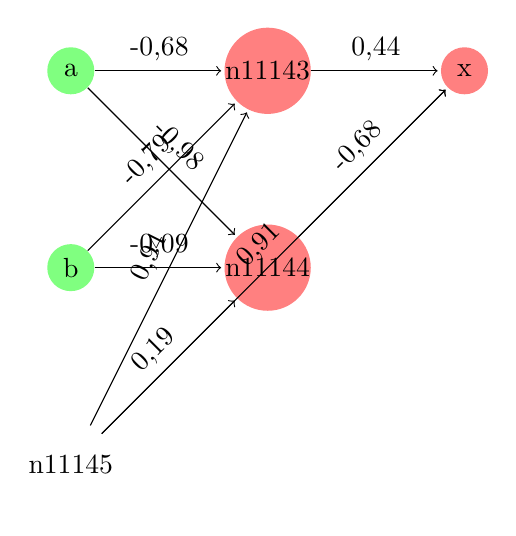
\begin{tikzpicture}[shorten >=1pt,->,draw=black!,node distance=2.5cm]
\tikzstyle{neuron}=[circle,fill=black!25,minimum size=17pt,inner sep=0pt]
\tikzstyle{constant}=[neuron, fill=white!50];
\tikzstyle{identity}=[neuron, fill=green!50];
\tikzstyle{sigmoid}=[neuron, fill=red!50];
\node [identity] (a) {a};
\node [identity,below of=a] (b) {b};
\node [constant,below of=b] (n11145) {n11145};
\node [sigmoid,right of=a] (n11143) {n11143};
\node [sigmoid,below of=n11143] (n11144) {n11144};
\node [sigmoid,right of=n11143] (x) {x};
\path[every node/.style={sloped,anchor=south,auto=false}]
(a) edge node {-0,68} (n11143)
(a) edge node {-0,98} (n11144)
(n11145) edge node {0,91} (x)
(n11145) edge node {0,19} (n11144)
(n11145) edge node {0,94} (n11143)
(n11143) edge node {0,44} (x)
(b) edge node {-0,79} (n11143)
(b) edge node {-0,09} (n11144)
(n11144) edge node {-0,68} (x)
;\end{tikzpicture}
\end{document}